

Our robot moves with two DC motors.In the simplest way, the DC motor speed is proportionnal to its
input voltage $U$.
Since we want to control the motor speed, we need to control the input voltage. An efficient and quite simple way to control this voltage is using Pulse Width Modulation (PWM).


\subsection{Pulse Width Modulation}
\UPSTIdefinition{
 The duty cycle is defined as  the fraction of one period in which a signal or system is active.
}
\begin{figure}[!ht]
 \centering
 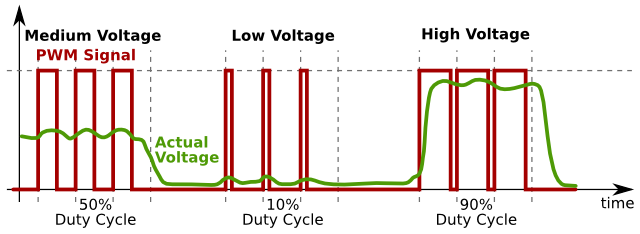
\includegraphics[width=.8\textwidth]{images/PWM_signal}
 \caption{PWM signal}
 \label{fig:PWM_signal}
\end{figure}
The idea is to make a high frequency signal and control its average value to the voltage value we want.

The higher the duty cycle is, the higher the signal average will be, as illustrated on Figure~\ref{fig:PWM_signal}.
If the duty cycle is \num{.5} (\SI{50}{\%}), the motor speed is at \SI{50}{\%} of its maximal value.

\pagebreak
\subsection{Controling the robot's motors : Full bridge}

To control the robot's motors we use a full bridge, illustrated on Figure~\ref{fig:schema_robot}.
As indicated in the table on Figure~\ref{fig:schema_robot}, \mintinline{C}{IN_1} and \mintinline{C}{IN_2} control the direction.
We control the speed by connecting the PWN to the \mintinline{C}{ENABLE} pin.

\begin{figure}[!ht]
 \centering
 \begin{subfigure}[b]{.7\textwidth}
  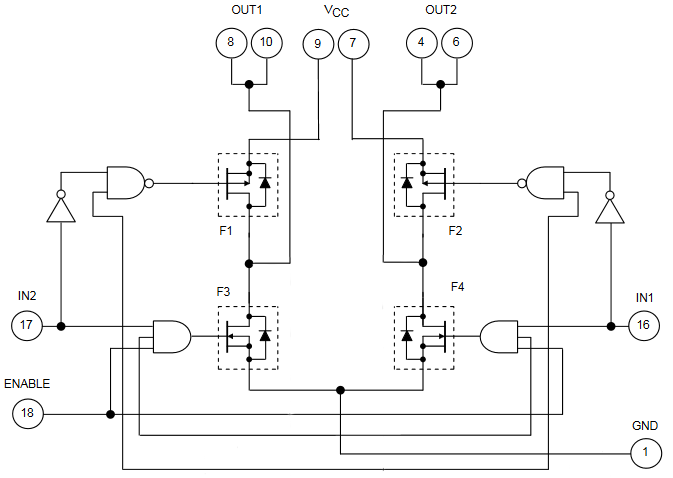
\includegraphics[width=\textwidth]{images/robot_schema}
  \caption{Schematic}
 \end{subfigure}

 \begin{subfigure}[b]{.7\textwidth}
  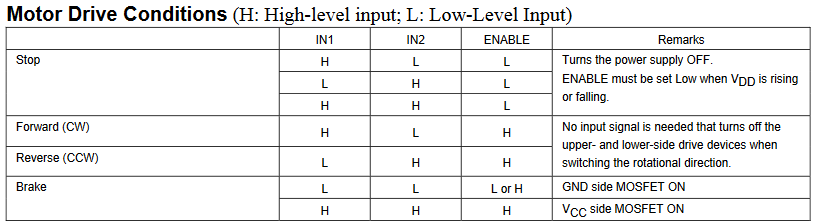
\includegraphics[width=\textwidth]{images/table_full_bridg}
  \caption{Control}
 \end{subfigure}
 \caption{Full bridge}
 \label{fig:schema_robot}
\end{figure}

\pagebreak
\subsection{Testing the motors}

For testing if the PWM controlling the motors is fully functionnal, we use the \mintinline{C}{ft_test_motor} function.
This function ask the user to define the wanted duty cycle and call the \mintinline{C}{ft_run_motor} function to run the PWM. You will implement this function to run the motors :

\inputminted[numbersep=4pt,linenos,firstline=11]{C}{programmes/ft_run_motor.cpp}
\begin{UPSTIactivite}[][Testing the motors][][][To do]
 \begin{enumerate}
  \item On the pinmap of the nucleo card (Figure~\ref{fig:right_connector} and Figure~\ref{fig:left_connector}), look for \textit{L. Mot Dir1}, \textit{L. Mot Dir2}, \textit{R. Mot Dir1} and \textit{R. Mot Dir2} and write the associated PIN.
  \item In the mbed compiler, edit the file \mintinline{C}{includes/pin_connexions.h}
        \begin{enumerate}
         \item Declare and connect the \mintinline{C}{DigitalOut} signals \mintinline{C}{DIR_1L, DIR_2L, DIR_1R, DIR_2R} to control the direction of left and right motor.
         \begin{itemize}
           \item \mintinline{Cpp}{DigitalOut DIR_1L (PC_9);}
         \end{itemize}
         \item Declare and connect the \mintinline{C}{PwmOut} signals \mintinline{C}{Pwm_ML and Pwm_MR} to control the PWM of each motor.
         \begin{itemize}
           \item \mintinline{cpp}{PwmOut Pwm_ML (PA_9);}
         \end{itemize}
        \end{enumerate}
  \item In the mbed compiler, edit the \mintinline{C}{Src/test_motor/ft_run_motor.cpp} file so that
        \begin{enumerate}
         \item Set the \mintinline{C}{dirA} and \mintinline{C}{dirB} value depending on the wanted direction,
         \item Set the PWM signal to the \mintinline{C}{duty_cycle} given in argument.
        \end{enumerate}
  \item Edit \mintinline{C}{main.cpp} to call \mintinline{C}{ft_test_motor} function:
        \inputminted[firstline=67,lastline=68]{C}{programmes/main.cpp}
        \inputminted[firstline=72,lastline=73]{C}{programmes/main.cpp}
 \end{enumerate}
\end{UPSTIactivite}
